
\index{itk::ImageToImageMetric|textbf}

In ITK, \code{itk::ImageToImageMetric} objects measures quantitively 
how well the transformed moving image fits the fixed image by comparing 
the grayscale intensity of the images. These metrics are very flexible
and can work with any transform or interpolation method and does not
require the reduction of the grayscale images to sparse extracted
information such as edges.

The metric component is perhaps the most critical element of the
registration framework. The selection of which metric to use is highly
dependent on the registration problem to be solved. For example, some metrics
have a large capture range while others require initialization close to
the optimal position; some metrics are only suitable for comparing 
images obtained from the same imaging modality while others can handle
inter-modality comparisions. Unfortunately, there are no clear-cut rules
as to how to choose a metric.

\index{itk::ImageToImageMetric!GetValue()}
\index{itk::ImageToImageMetric!GetDerivatives()}
\index{itk::ImageToImageMetric!GetValueAndDerivatives()}

The basic inputs to a metric are: the fixed and moving images, a
transform and an interpolator. The method \code{GetValue} can
then be used to evaluate the quantitive criterion at the transform
parameters specified in the argument. Typically, the metric samples 
points within a defined region of the fixed image. 
For each point, the corresponding moving image position is
computed using the transform with the specified parameters, 
then the interpolator is used to compute the moving image intensity 
at the mapped position.

As well as the measure value, gradient-based optimization schemes also require
derivatives of the measure with respect to each transform parameter. The
methods \code{GetDerivatives()} and \code{GetValueAndDerivatives()} can be used
to obtained the gradient information.


Metrics currently available in ITK are:
\begin{itemize}
\item Mean Squares
\item Normalized Correlation
\item Mutual Information
\item Pattern Intensity
\end{itemize}
In the following sections, we describe each metric type in detail. 
For ease of notation, we will refer to the fixed image $f(\bf{X})$ 
and transformed moving image $m \circ T(\bf{X})$ as images $A$ and $B$.

\subsection{Mean Squares Metric}
\label{sec:MeanSquaresMetric}
This metric computes the mean square pixel-wise difference in intensity
between image $A$ and $B$ over a user defined region:

\begin{equation}
MS(A,B) = \frac{1}{N} \sum_i^N \left( A_i - B_i \right)^2
\end{equation}
\begin{center}
$A_i$ is the i-th pixel of Image A\\ 
$B_i$ is the i-th pixel of Image B\\
$N$ is the number of pixels considered
\end{center}

The optimal value of the metric is zero. Poor matches between images
$A$ and $B$ results in large values of the metric. This metric is
simple to compute and have a relatively large capture radius.

This metric relies on the assumption that intensity representing
the same homologous point must be the same in both images. Hence,
its use is restricted to images of the same modality. Additionally,
any linear changes in the intensity result in a poor match value.

\subsection{Normalized Correlation Metric}
\label{sec:NormalizedCorrelationMetric}
This metric computes pixel-wise cross-correlation and normalize it
by the square root of the autocorrelation of the images:

\begin{equation}
NC(A,B) = \frac{ \sum_i^N \left( A_i \cdot B_i \right) }
         { \sqrt { \sum_i^N A_i^2  \cdot \sum_i^N B_i^2 } }
\end{equation}
\begin{center}
$A_i$ is the i-th pixel of Image A\\ 
$B_i$ is the i-th pixel of Image B\\
$N$ is the number of pixels considered
\end{center}

The optimal value of the metric is one. Misalignment between the
images results is small measure values. The use of this metric
is limited to obtained using the same imaging modality. The metric
is insenstive to multiplicative differences between the two
images. This metric produces a cost function with sharp peaks and well
defined maxima. On the other hand, it has a relatively smaller
capture radius.

\subsection{Pattern Intensity Metric}
\label{sec:PatternIntensityMetric}
This metric computes pixel-wise differences and add them 
after passing them through a bell-shaped function $\frac{1}{1+x^2}$:

\begin{equation}
PI(A,B) =  \sum_i^N \frac{ 1 }{ 1 + \lambda \left( A_i - B_i \right) ^ 2 }
\end{equation}
\begin{center}
$A_i$ is the i-th pixel of Image A 
$B_i$ is the i-th pixel of Image B
$N$ is the number of pixels considered
$\lambda$ controls the capture radius
\end{center}

The optimal values is $N$ and poor matches results is small measure
values.

Advantages
\begin{itemize}
\item Produce poor values when few pixels are considered
\item Capture radius can be controled
\item Profile is very pointy (high precision)
\end{itemize}

Disadvantages
\begin{itemize}
\item Limited to same image modality
\item Its derivative is high at the peak this is a problem for some optimizers
\item Sensitive to linear changes in intensity
\end{itemize}


\subsection{Mutual Information Metric}
\label{sec:MutualInformationMetric}
This metric computes the mutual information between image $A$ and image $B$.
Mutual information (MI) measures how much information one random variable
(image intensity in one image) tells about another random variable 
(image intensity in the other image). The major advantage of using
MI is that the actual form of the dependency does not have to be specified. 
Therefore, complex mapping between two images can be modeled. 
This flexibility makes MI well suited as a criterion of multi-modality
registration.

Mutual information is defined in terms of entropy. Let
\begin{equation}
H(A) = - \int p_A(a) \log p_A(a)\, da
\end{equation}
is the entropy of random variable $A$, $H(B)$ entropy of 
random variable $B$ and 
\begin{equation}
H(A,B) = \int p_{AB}(a,b) \log p_{AB}(a,b)\,da\,db
\end{equation}
be the joint entropy of $A$ and $B$.

If $A$ and $B$ are independent then
\begin{equation}
p_{AB}(a,b) = p_A(a) p_B{b}
\end{equation}
and
\begin{equation}
H(A,B) = H(A) + H(B).
\end{equation}
However, if there is any dependency then
\begin{equation}
H(A,B)<H(A)+H(B).
\end{equation}
The difference is called Mutual Information : \( I(A,B) \)
\begin{equation}
I(A,B)=H(A)+H(B)-H(A,B)
\end{equation}


Computes how much uncertainty about one image can be
reduced by having the information contained in the other
image.

Information == Reduction in uncertainty

\begin{equation}
H(A)=-\sum _{i=1}^{G}p(a_{i})\cdot \log p(a_{i})
\end{equation}

\begin{center}
$a_{i}$ is the i-th gray level of image A
$G$ is the number of gray levels in image A
$p(a_{i})$ is the probability of finding $a_{i}$ in a pixel of A
\end{center}

\begin{equation}
H(A) = \mbox{Entropy of} A
\end{equation}

$p(a_{i})$ values can be estimated from the image histogram.

A population of pixel pairs can be obtained by taking homologous pixels from
two images.

Joint Entropy can be computed from the statistical distribution of gray levels.

\begin{equation}
H(A,B)=-\sum _{i=1}^{G_{A}}\sum _{j=1}^{G_{B}}p\left( a_{i},b_{j}\right) \cdot \log p\left( a_{i},b_{j}\right)
\end{equation}


\begin{center}
$a_{i}$ is the i-th gray level of image A
$b_{j}$ is the j-th gray level of image B $p\left( a_{i},b_{j}\right)$ is the
probability of finding the gray level $a_{i}$ associated with the gray level
$b_{j}$ in the same pair of pixels.
\end{center}


If the gray levels of A are independent of B

\begin{equation}
p\left( a_{i},b_{j}\right) =p\left( a_{i}\right) \cdot p\left( b_{j}\right) 
\end{equation}


and then 

\begin{equation}
H(A,B)=H(A)+H(B)
\end{equation}


but if there is any dependency

\begin{equation}
H(A,B)<H(A)+H(B)
\end{equation}


the difference is called Mutual Information : \( I(A,B) \)

\begin{equation}
I(A,B)=H(A)+H(B)-H(A,B)
\end{equation}


\subsubsection{Parzen Windowing}

The probability distributions of gray levels are in general unkown.

They can be estimated by taking samples (pixels) from the image and
reconstructing a continuous function by convolving the samples with a smoothing
kernel function.

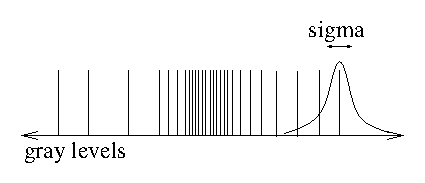
\includegraphics{ParzenWindowing1.eps}

This is typically done with a Gaussian. A value of sigma should be selected
somehow related with the number of pixels sampled.  

\subsubsection{Convolution with the
smoothing function}

\resizebox*{0.5\columnwidth}{!}{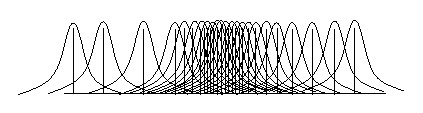
\includegraphics{ParzenWindowing2.eps}}

Resulting continuous probability distribution 

\resizebox*{0.5\columnwidth}{!}{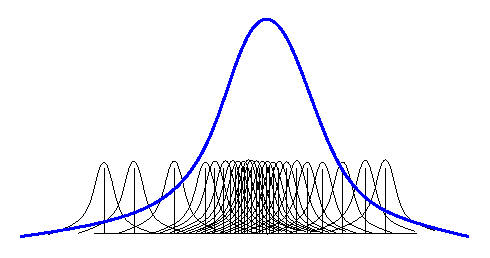
\includegraphics{ParzenWindowing3.eps}}


Advantages

\begin{itemize}
\item Allows to compare different image modalities
\item Few samples (pixels) are required
\end{itemize}

Disadvantages

\begin{itemize}
\item Requires to tune parameters (number of samples and parzen windowing probability distributions estimation)
\item Not suitable for images related by linear relationships
\end{itemize}





